\chapter{Mint}

Prior to the development of the summarization system, it was important to develop a sense for what is really need from such a system, and what problems can it really solve. To answer these quesitons, I developed an Aeolus application based on the financial management service \emph{mint.com}. The \emph{Mint} application served as a case study and guided the development of the summarization system.

In this chapter I present the Mint application model as well as some examples to how a summarization system could be used for this application.

\section{Mint Model}

Mint.com is an financial management service that provides it's users with the ability to monitor their bank accounts across different banks from one place. It also allows Mint users to run transaction analysis tools that will access the information of certain transactions for each bank for the user, and generate a result.

For example, Bob could sign up on www.mint.com and add his Bank of America account and his US Bank account for monitoring. Bob can then request a graph that presents his expenditures on food in the last week.

In this section we examine the security model of the application more closely.

\subsection{Authority State Model}

In this section we identify the prinicpals running in the system, the tags associated with different data, and the relationships between them.

A very intuitive way to list all necessary\footnote{Neccessary by good design. The application could run with just one principal} principals, is to think of the different ``clearance levels'' in the system: some information should be accessible by a user, some by a bank, and some information should not be accessible at all. In the light of these requirements, the application employs the following principals:
\begin{description}
  \item[Mint principal] \ \\
    This principal is authoritative for all tags in the system.
  \item[Bank principals] \ \\
    Each of these principals is authoritative for a particular bank's tag.
  \item[User principals] \ \\
    Each of these principals is authoritative for a particular user's tag.
  \item[Public principal] \ \\
    This prinicpal is not authoritative for any tags 
    \footnote{It is used when no privileged operations 
      are necessary to ensure that no information leaks}.
\end{description}

Similarly, to separate data in the system according to it's purpose, (e.g. user password, credentials to download bank transactions, etc..), the application employs the following tags:
\begin{description}
  \item[User tags] \ \\
    Each of these tags is associated with data 
    carrying a particular user's information.
  \item[Bank tags] \ \\
    Each of these tags is associated 
    with data carrying a particular bank's information.
  \item[All-Users-Data tag] \ \\ 
    This tag is a super tag for all the user 
    tags.
  \item[All-Banks-Data tag] \ \\ 
    This tag is a super tag for all the bank tags.
\end{description}

The following two sections explain how data is stored in the system and how tag which tag operations are carried out in a typical workflow.

\subsection{Files and Shared Memory Objects}

The application uses Aeolus' file system API, for persistent storage, and uses Aeolus shared memory objects for storing session state for users and bank closures. A complete description of the Aeolus file system API is presented by McKee \cite{mckee}.

\subsubsection{Files}\label{fs}

The application stores it's information under a root directory called \emph{mint-dir}. The are two direct subdirectories of $mint-dir$: \emph{banks-dir} and \emph{users-dir}.

$banks-dir$ contains a file for each bank the application supports, the filename is derived from the bank name. $users-dir$ contains a subdirectory per user, each of these subdirectories contains two files for the user called \emph{user-info} and \emph{user-password} as well as another file per bank the user has added, called \emph{user-bank-info}.

$user-info$ contains the user tag for that user. $user-password$ contains the user's password. $user-bank_name-info$ contains the credentials for the user to authenticate with a specific bank. Figure x shows a sample directory tree, and table x shows the file labels.

\subsubsection{Shared Memory}

To allow for quick responsiveness to user requests, the application stores some key information in shared memory:

\begin{description}
  \item[Bank closures] \ \\
    Bank closures are objects that allow the application to connect to the bank 
    and retrieve user information. Storing them in memory allows for a quicker 
    response if a user's request requires connecting to a bank. It is not very 
    costly to store them in memory because the number of banks supported by 
    the server is limited. 
  \item[Session Objects] \ \\
    Session objects contain session information about a user. They are stored in a
    map that maps a session-id to a session object. The session object contains 
    the list of the bank credentials a user has registered, as well as the 
    user's PID.
  \item[User tags] \ \\
    The application stores the tag for each user that has an active session, this
    allows the application server to access session objects with the user tag in 
    their label. User tags are stored as a mapping from username to tag.
  \item[Bank tags] \ \\
    Bank tags are important to store in memory to allow for quick server 
    response time. They are stored as a map from bank name to bank tag.
  \item[User idle time] \ \\
    User idle time identifies users that are still active. This information is 
    stored as a mapping form username to last activity time.
\end{description}

\section{Implementation}

The application server runs on a virtual node, and receives user requests via RPC\footnote{HTTP requests would be more suitable for this purpose, but the application enforces that the RPC requests have null labels, and hence it is as if they are received from outside the system. The difference then between using RPC or HTTP becomes purely a matter of implementation}. 
Users can sign up, login, logout, register a bank, retreieve statistics as well as \emph{attack other users}.

User requests spawn a thread at the server that runs as the Mint principal. The thread first loads the server state from memory, then the thread authenticates the user, carries out the requested user action and returns. This requires label manipulation, reading from and writing to disk, and accessing shared memory storage. The following section describes the authentication mechanism as well as each user action in more detail.

\subsection{Authentication and User Actions}

Users sign up to the service by sending a \emph{signUp} RPC to the server. The server then creates a PID and a tag for that user, and stores this information, along with user credentials, on disk as described in seciton~\ref{fs}.

A user of the Mint application starts a session by logging in. The system authenticates the credentials by calling an authentication closure, which adds the All User Data tag, verifies the credentials, declassifies and returns the result of the verification.

Once a user logs in, they use a session id to authenticate their future requests. To authenticate session ids, the system accesses the shared memory objects described above to verify that the user's session has not timed out.

If authentication is successful, the thread carries on and executes the user's request. We now examine the different user actions the application supports.

\begin{description}
  \item[\emph{signUp(username, password)}] \ \\
    Signs up a new user with the username as \emph{username} and 
    password as \emph{password} if \emph{username} is available, and associates
    those credentials with a tag and a principal ID.
    The label modifications happen as described above.
  \item[\emph{login(username, password)}] \ \\
    Authenticates a user, and if successful, places their information in shared 
    memory. Label manipulation happens as described above. Following requests from
    this user only need to include the username.
  \item[\emph{logout(username)}] \ \\
    Terminates the user's session, removing their information from shared memory.
  \item[\emph{addBank(username, bankName, bankCredentials)}] \ \\
    Registers the specified bank for the specified username with the given 
    credentials.
    This request writes a \emph{user-bank-info} file to disk, with the tag of
    the user in it's integrity label, and the tag of the user and that of the bank
    in it's secrecy label.
  \item[\emph{removeBank(username, bankName)}] \ \\
    Removes the specified bank from a user's account.
  \item[\emph{downloadTransactions(username)}] \ \\
    This action connects to each bank the user has registered on their account, 
    downloads the latest transactions, processes them and returns the result.
    The RPC thread uses a closure call that runs with the PID of the bank to
    connect to the bank and declassify the information returned. The thread then
    adds a user tag to it's secrecy label, and uses a reduced authority call to 
    public principal to process the information, this ensures that information
    cannot be leaked while it is being processed\footnote{One can imagine that the 
    information is being processed by a different application in the system, 
    using this technique means our application does not have to trust that 
    application. Only the code for the Bank closure needs to be trusted.}. After
    that the thread declassifies and returns. Figure x shows a code sample.
  \item[\emph{attack(attacker, victim)}] \ \\
    \emph{Attacks} the uer specified by \emph{victim}. This request aims to 
    simulate a bug in the appliction that mistakingly delegates the victim's 
    data tag to the attacker's principal.
    This user action is useful for testing and auditing purposes, as explained later
    in this chapter.
\end{description}

Figures: closure code sample, authority state structure, file system tree + labels, auditing + summarization

\section{Auditing and Summarization}
\label{mint:auditing}
The application makes use of the Aeolus audit trails system described in \cite{popic} and \cite{blanks} to monitor system behavior. In particular, we monitor label modification involving a particular user's data tag. Figure x shows a table of which principals declassified Bob's tag, in other words, it shows which user's accessed Bob's information. Figure \ref{figure:activity} shows a graph of how many user requests caused a label modifications involving a user data tag for every 5-second period since the application launched, in other words, it shows the activity trend of the user, any spikes in the graph mean that the user was abnormaly active in certain periods of time, which could raise suspicion to their account being compromised.


\begin{figure}
\centering
\includegraphics[scale=0.85]{figures/activity.eps}
\caption{This graph shows the activity trend of each user. Notice that the activity for user Jack spikes in the graph at multiple places, this could be the result of an attacker accessing his account and issuing many requests to retreieve all of Jack's financial information in a short amount of time.}
\label{figure:activity}
\end{figure}
In this section we described how the data for Figure x can be extracted from the event log, as well as the possible uses of summarization for this scenario.

\subsection{Logging}

Aeolus provides a library that allows application developers to add their own application-specific events to the event log. These events are meant to help the developer attach semantic meaning to the event records in the log.

In order to gather the information necessary to produce the graph in figure x, we add application-specific event records to the event log for each different action the user takes.

For example, when a user signs up successfully with our application, we record their username, as well as the tag and principal associated with this user. This done using the following procedure:

\begin{lstlisting}[language=Java]
  AeolusLib.createEvent(``mint-signup'', username, principal, tag);
\end{lstlisting}

In order to obtain a table detailing the username, prinicpal, data tag and other sign-up information of all users, we create a view based on our application-specific events using the following SQL query\footnote{\emph{to\_array} is a procedure that turns a comma-delimited string into a PSQL array.}:

\begin{lstlisting}[language=SQL, deletendkeywords={TIMESTAMP}]
create view users as select to_array(app_arg)[0] as pid, to_array(app_arg)[1] as username, to_array(app_arg)[2] as tag, timestamp as signed_up, event_counter from events where op_name='mint-signup'
\end{lstlisting}

Table \ref{table:users-info} shows what such a view would look like, with some extra information about time of when each user signed up. We can now use this table to extract more semantic information about the event log.

\begin{table}
\begin{verbatim}

 pid | username | tag  |        signed_up        | event_counter 
-----+----------+------+-------------------------+---------------
   6 | wissam   | [4]  | 2012-06-13 21:56:36.207 |           131
   9 | david    | [7]  | 2012-06-13 21:56:36.207 |           445
  12 | dan      | [10] | 2012-06-13 21:56:37.338 |           793
  13 | Bob      | [11] | 2012-06-13 21:56:37.338 |          1148
  14 | Charlie  | [12] | 2012-06-13 21:56:37.338 |          1211
  15 | Eve      | [13] | 2012-06-13 21:56:37.338 |          1274
  16 | Ted      | [14] | 2012-06-13 21:56:37.338 |          1337
  17 | Jon      | [15] | 2012-06-13 21:56:37.338 |          1400
  18 | Jack     | [16] | 2012-06-13 21:56:37.338 |          1463
  19 | James    | [17] | 2012-06-13 21:56:37.338 |          1526
  20 | Mike     | [18] | 2012-06-13 21:56:37.338 |          1589
  21 | Mark     | [19] | 2012-06-13 21:56:37.338 |          1652
  22 | Jamie    | [20] | 2012-06-13 21:56:38.578 |          1715
  23 | Dave     | [21] | 2012-06-13 21:56:38.578 |          1778
  24 | Tod      | [22] | 2012-06-13 21:56:38.578 |          1841
  25 | Chris    | [23] | 2012-06-13 21:56:38.578 |          1904
  26 | Ron      | [24] | 2012-06-13 21:56:38.578 |          1967
  27 | Phil     | [25] | 2012-06-13 21:56:38.578 |          2030
  28 | Tracy    | [26] | 2012-06-13 21:56:38.578 |          2093
  29 | Leah     | [27] | 2012-06-13 21:56:38.578 |          2156
  30 | Kevin    | [28] | 2012-06-13 21:56:38.578 |          2219
  31 | Rose     | [29] | 2012-06-13 21:56:38.578 |          2282
  32 | Dina     | [30] | 2012-06-13 21:56:38.578 |          2345
  33 | Abby     | [31] | 2012-06-13 21:56:38.578 |          2408
  34 | Helen    | [32] | 2012-06-13 21:56:38.578 |          2471
  35 | Alex     | [33] | 2012-06-13 21:56:38.578 |          2534
  36 | Aline    | [34] | 2012-06-13 21:56:38.578 |          2597

\end{verbatim}
\caption*{Users Table}
\caption{This is a table detailing the information of users signing up during a simulated run of the Mint application. The \emph{pid} column denotes the user's principal, the \emph{username} column denotes the user's username, the \emph{tag} column denotes the user's data tag, the \emph{signed\_up} column denotes the time at which the sign up event was logged to the system, and the \emph{event\_counter} column denotes the unique event\_counter number of the sign up event. }
\label{table:users-info}
\end{table}

For example, we can obtain the information necessary to create the graph in figure y using this query:

\begin{lstlisting}[language=SQL, deletendkeywords={TIMESTAMP}, label=query:accesses]
create view accesses as select e.count, users.username, e.to_timestamp as timestamp from (select count(*), tags_modified, (to_timestamp(((extract (epoch from events.timestamp)/5)::int)*5)) from events tags_modified in (select tag from users) group by (to_timestamp(((extract (epoch from events.timestamp)/5)::int)*5)), tags_modified) as e inner join users on e.tags_modified=users.tag
\end{lstlisting}

Table \ref{table:activity} shows a sample result of this query. This query provides us with a count of how many user requests requests caused a label modification that involved a user data tag for every 5-second period of time since the application launch, the information necessary to construct the graph in figure y.

\begin{table}
\begin{quote}
\begin{verbatim}
 count | username |       timestamp        
-------+----------+------------------------
    22 | Jack     | 2012-06-13 21:56:40-04
     4 | Jack     | 2012-06-13 21:56:35-04
    42 | Jack     | 2012-06-13 21:56:50-04
    72 | Jack     | 2012-06-13 21:57:00-04
    90 | Jack     | 2012-06-13 21:56:45-04
    12 | Jack     | 2012-06-13 21:56:55-04
    22 | Jack     | 2012-06-13 21:57:05-04
\end{verbatim}
\end{quote}
\caption*{Account activity for user \emph{Jack}}
\caption{This table shows a sample result of the \emph{accesses} view (for simplicity we only show the result for the user Jack). It details the number of user requests causing a label manipulation involving a user data tag for every 5-second period since the application launched. The \emph{count} denotes such number. The \emph{username} column denotes the user who's data tag is in question. The \emph{timestamp} column denotes the start of the 5-second period.}
\label{table:activity}
\end{table}

\subsection{Study Case for Summarization}

One of the main purposes of building this application was to evaluate how developers would go about auditing the events in the system, and what can be done to make that task easier. In the next chapter we describe the issues we identified and how our summarization system resolves them.
